
\chapter{Preliminary work on slice creation and tagging}
\setcounter{page}{1}
\renewcommand{\thepage}{\Alph{chapter}--\arabic{page}}

This work, namely \autoref{chap:methods}, was devoted to a thorough study of the performances of Pandora event reconstruction targeting a specific topology of events, and focusing on the part of the chain that focused on the reconstruction of the neutrino interaction, PandoraNeutrino. 

A equally important step of Pandora event reconstruction 

\section{Slice creation and tagging}

All these algorithms are part of the PandoraNeutrino reconstruction path, with both the 2D clustering and the 3D reconstruction stages also implemented in the PandoraFastReco and PandoraCosmic reconstruction paths. The PandoraFastReco is crucial, as part of the reconstruction chain, to perform a ``fast reconstruction'', allowing the slice creation tools to create the interaction slices. 

% why is slice creation core to the reconstruction?
Since this stage is run upstream of the PandoraNeutrino reconstruction path, ensuring a correct creation of the slices is core for the success of the subsequent reconstruction steps. As a matter of fact, if the slicing process fails and for some reason splits one interaction in half, the following reconstruction steps cannot recover the underlying interaction, even if cheating all the stages of the PandoraNeutrino reconstruction (i.e., making the reconstruction downstream of the slice creation ``perfect''). \autoref{fig:slicingIssue} shows this case with an example. In the figure, a $\PGnGm$CCQE Np event is shown. All the hits in the interaction are shown in the last panel. When the slice creation tool is run, however, it splits the prompt muon into two separate slices (Slice A/B, third and fourth panels). Then, performing the fully cheated reconstruction, thus effectively showing the underlying true particles in the interaction (Slice A/B, first two panels), reveals that what will be selected as a true and reconstructed $1\PGm1\Pp$ slice is Slice A. Slice B contains only half of the muon track and the muon decay Michel electron. 

%% issues (figure)
\begin{figure}[!htb]
    \centering
    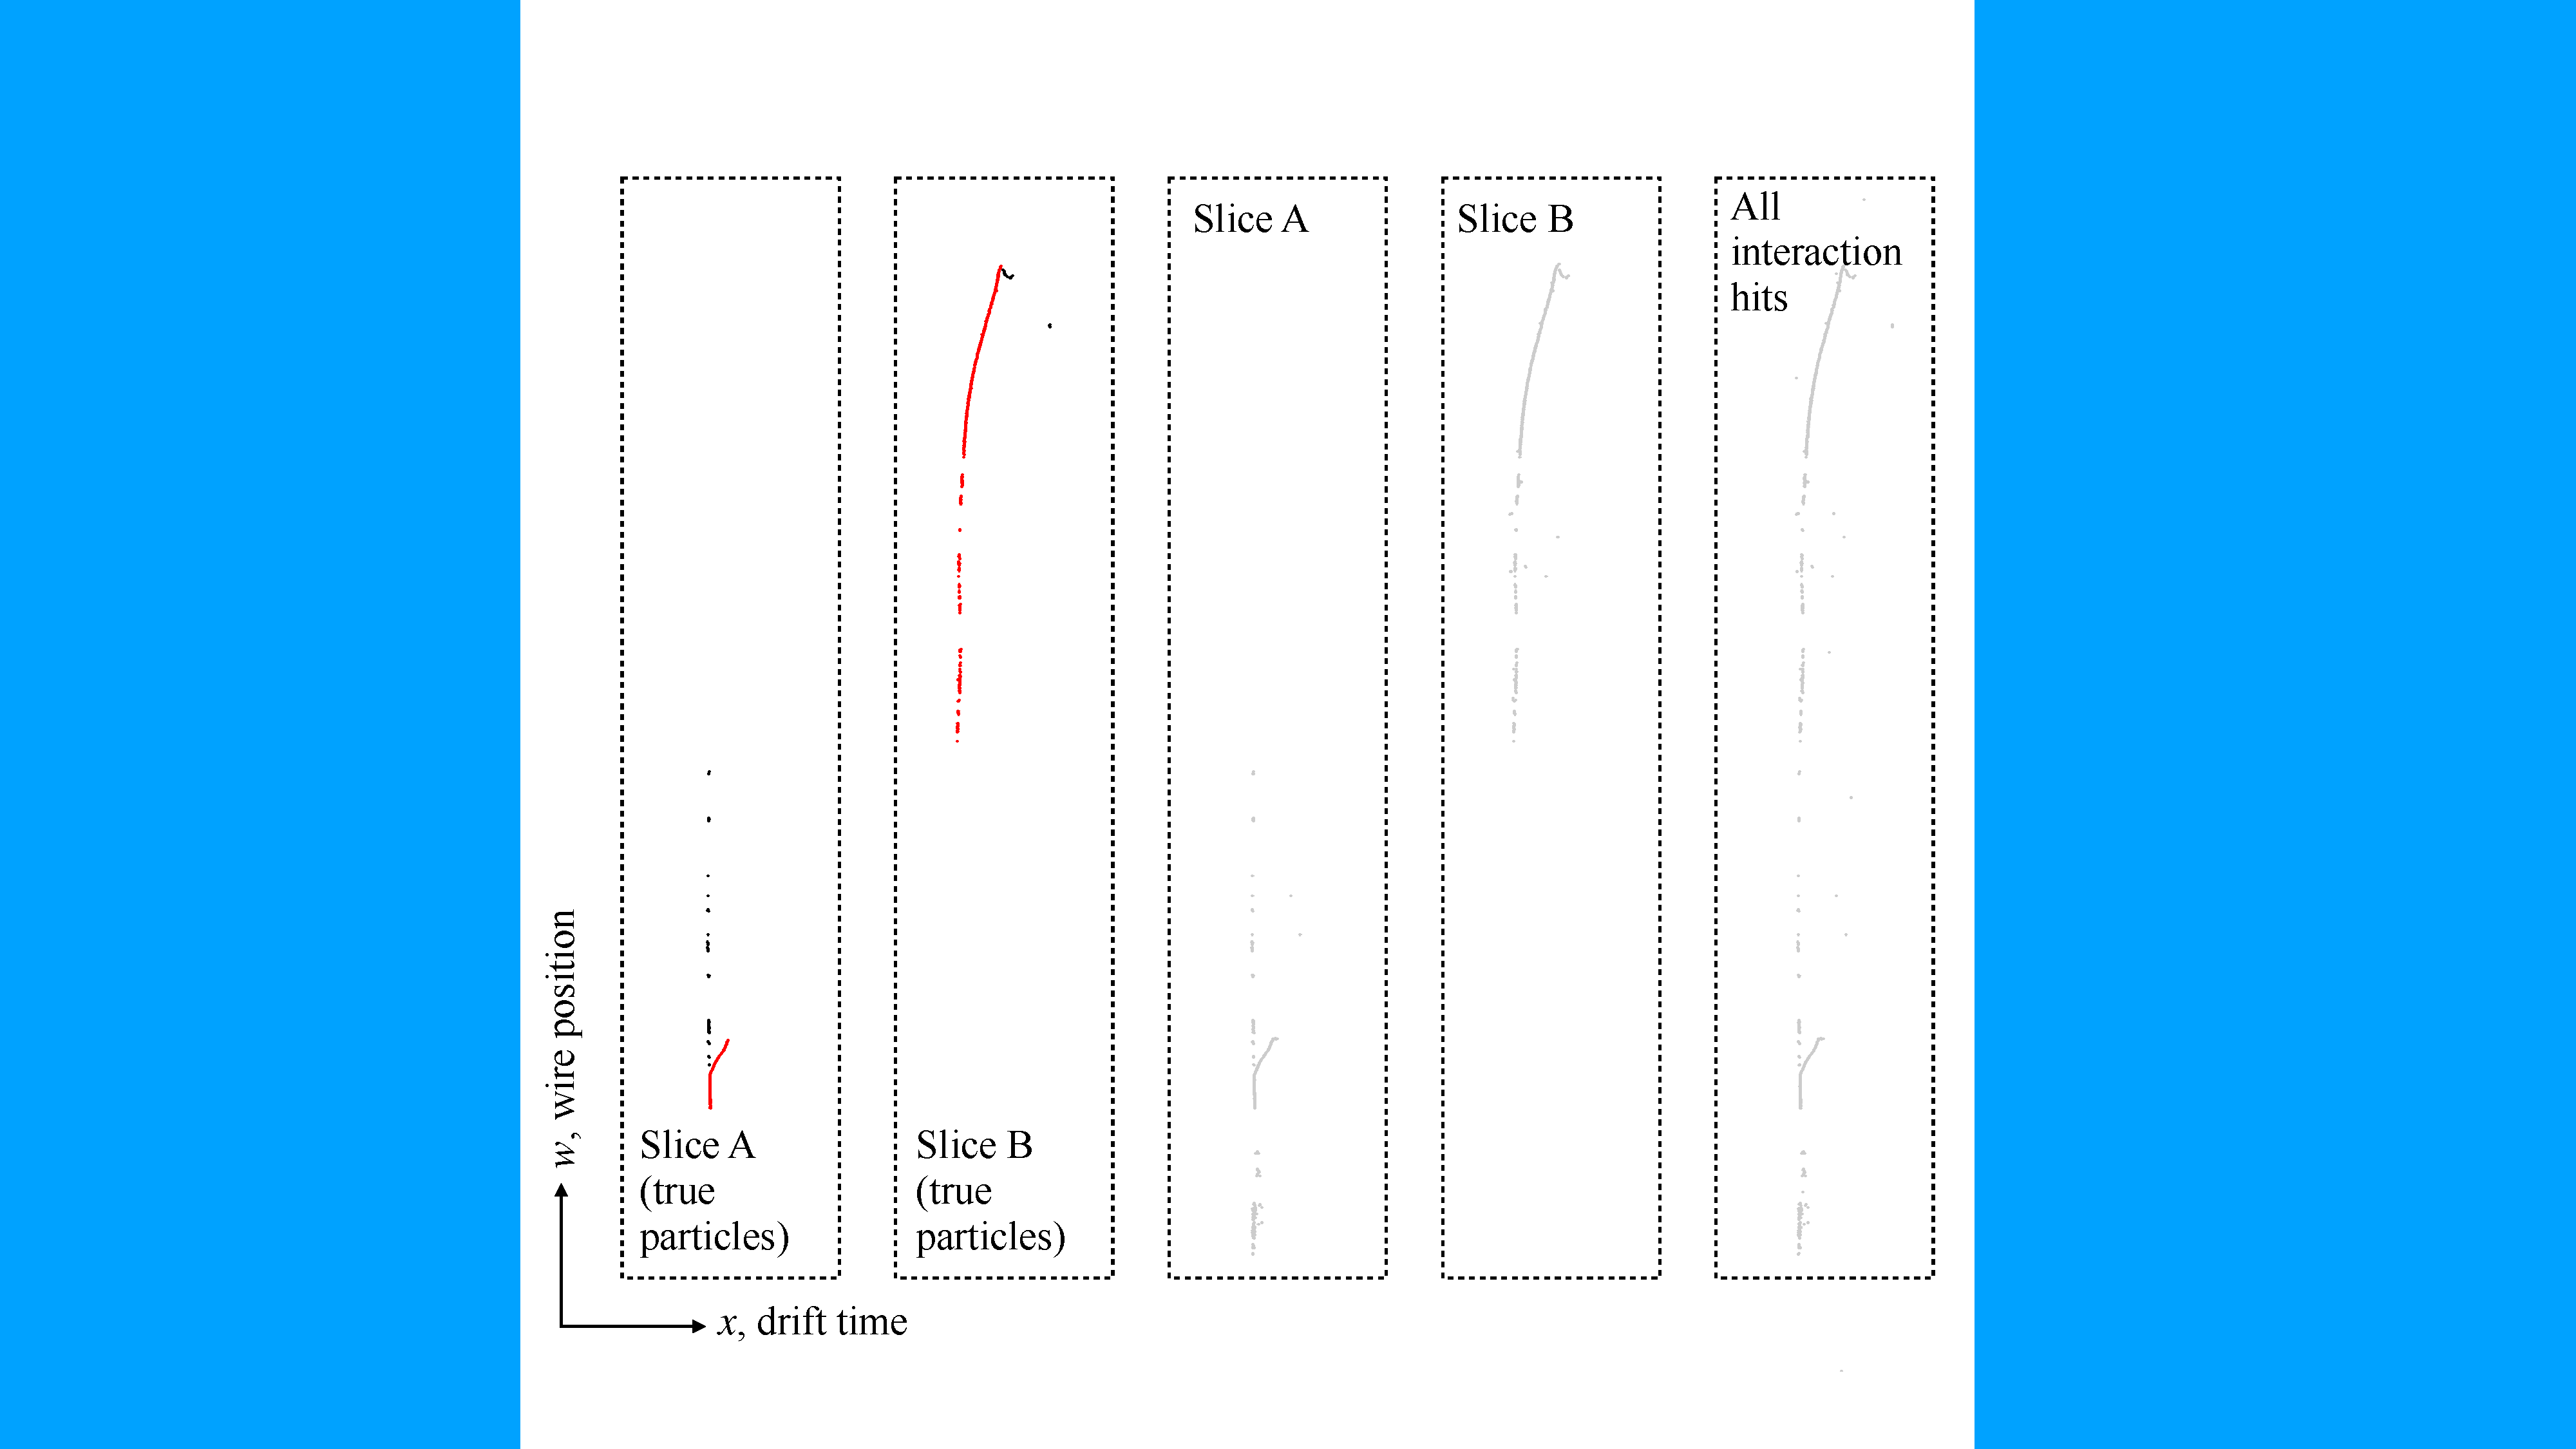
\includegraphics[width=0.95\linewidth, trim={14cm 0 16cm 0}, clip]{pandora/chapter_4/slicing.pdf}
    \caption[Slice creation failure mode]{Example of an event where the slice creation tool failed to correctly create one slice for the interaction, splitting it instead into two separate slices. }
    \label{fig:slicingIssue}
\end{figure}

% how this tool is implemented
Since discovering that this was not an isolated case, the cheating of the slice creation tool was also considered. The working principle of the cheated slice creation tool is pretty straightforward. This looks at all the reconstructed hits in the events and associates them with the correct MC particles, which are arranged in the interaction with the correct hierarchy. Using the underlying MC information, this tool can therefore divide the hits on all three of the readout planes by the underlying interaction. These lists of hits divided by MC interaction are then used to have the downstream reconstruction performed on them. 